\documentclass[12pt]{article}
 
\usepackage{multirow}
\usepackage{geometry}
\geometry{a4paper, margin=1in}
\usepackage{titlesec}
\usepackage{lipsum} % For placeholder text, remove this in your actual document
\usepackage{graphicx}
\usepackage{float}
\usepackage{amsmath}
\usepackage{titlesec}
\usepackage{hyperref}
\usepackage{enumitem}
\usepackage{tabularx}
\usepackage{longtable}
\usepackage{multirow}
\usepackage{multicol}
\usepackage{array}     % For better column formatting

% \usepackage[style=authoryear-comp, backend=biber]{biblatex}
% \addbibresource{refernece.bib}
\titleformat{\section}[block]{\filcenter\bfseries\Large}{\thesection.}{1em}{}


% Set the subsection title format
\titleformat{\subsection}
{\normalfont\large\bfseries}{\thesubsection}{1em}{}

\begin{document}

\title{Hariom Mewada BPS2 Weekly Report}
\author{Hariom Mewada\\
24M2137}
\maketitle

\newpage
\tableofcontents
\newpage

\section{Feb 02 2026 - Feb 07 2026}
\subsection{To Do}
\begin{enumerate}
    \item Create plan for BPS2.
    \item Read some papers related to digital well being, try to find out gapes.
    \item Modify the app according to the future plan: Commertial tool or just a research prototype.
    \item Try to have some behavior change result from the app.
    \item If the result are promising then try some conferences to publish a paper on this work.
\end{enumerate}
\subsection{Proposed Changes to the existing system}
\begin{enumerate}
    \item  Deploy the existing app on play store.
    \item Refine the UI elements to correctly reflect the underlying psychology.
    \item Improve app's accuracy and performance as part of RA work.
    \item Make the system more secure.
\end{enumerate}
\subsection{Summary: Navigating Digital well-Being in Digital era: A scoping review of digital-wellbeing \cite{Zhao2024DigitalWellbeing}}|
\begin{enumerate}
    \item Most people across generations perceive frequent internet use as normal and acceptable.
    \item This study is a scoping review to identify, analyze, and synthesize existing definitions, measurements tools, and intervention strategies related to Digital well-Being(DWB).
    \item  Research emerging from \textbf{Asia} is scarce
        \item Existing Definition coverage on three perspectives:
        \begin{enumerate}
            \item DWB as emerging concept of well being influenced by technology use.
            \item As a perceived impact of digital engagement on individual well-being.
            \item As a balance use strategy within digital environment.
        \end{enumerate}
        \item Three overarching themes were synthesized -- behavioral intention to use technology, eudaimonic well being, and socio culture contextual factor.
        \item Measurement tool for DWB remains limited; with high five scales identified but none offering an integrated framework, interventions, particularly that emphasize on digital disconnection, reveal mixed result about their effectiveness.
        \item Collectively these findings highlights ambiguities, limited measurement development, and inconsistent intervention outcome.
        \item This review advances theoritical clarity by framing DWB as a multi dimensional construct that bridges pyschological and socio technological domain.
        \item It also provide practical guidance for developing culturally adaptive interventions and policy frameworks that promote balanced and meaningful digital engagement.
    \end{enumerate}
\subsection{Detaied Summary}
\begin{enumerate}
    \item According to \textbf{Data Reportal 2024} \cite{datareportal2024digital}, the number of internet user increased by \textbf{3.2 \% } from previous year, reaching \textbf{5.56 billion } user in \textbf{2024}. 
    \item This  figure represents \textbf{67.9 \%} of the global population, although reporting delay suggest that the actual penetration rate is even higher.
    \item The avg duration of daily internet usage has grown streadily, reaching \textbf{6h 38 min} .
    \item Internet engagement spans all age groups, though usage tends to decline over age.
    \item Digital devices now enable continous interaction anytime and anywhere, However constant connectivity often generate discomfort or a sense of loss when disconnected -- a phenomenon of called technological unconsciousness.
    \item (Hoehe and Thibaut 2020 )\cite{hoehe2020going} emphasized that individuals must be intentional, creative, and mindful in their technology use to enhance relationships and producitivy; otherwise, technology risks eroding rather than supporting.
    \item   As (Hoehe and Thibaut 2020) \cite{hoehe2020going} noted, technology itself is value neutral -- it can be beneficial or harmful depending on how it is applied.
    \item When technology intented to improve life is used without restrain than it can 
    ultimately reduce quality of life.
    \item Since quality of life is closed tied to well-being \cite{upton2015quality}  \cite{weil1997technostress} scholars have begun to recognize the need of a new construct -- \textbf{digital well being} -- to describe well being in the digital age.
    \iten Yet how individual conceptualize and experience digital wellbeing(DWB) remains insufficiently understood \cite{nguyen2022everyday}.
    \item The emergence of the term \textbf{digital - well being } reflects a broader historical evolution in how societies interpret the relationship between technology and quality of life.
    \item Early scholarship on intrernet addiction \cite{kraut1998internet} technostress \cite{tarafdar2007technostress} laid the conceptual groundwork by examining the psychological costs of rapid oraganization.
    \item This study highlighted the paradox of technological progress -- it's simulatenous capacity to enhance connectivity and generate new form of strain.
    \item Building upon this foundation the notion of Digital well being emerged in in late \cite{2010} as scholars and industry leaders sought to redefine a healthy relationship.
    \item Major corporate initiative further popularized the concept . Google's \textbf{Digital wellbeing} and Apple's \textbf{Screen Time} programs, for instance framed digital balance as design priority, emphasizing user awareness and self regulation.
    \item This industry efforts marked a pivotal shift from merely preventing overuse to actively designing for well-being, signaling a convergence between technology ethics, public health, and user centric innovation.
    \item Thus DWB represents both academic and applied response to evolving socio-technical landscape -- bridging earlier studies on technostress  and contemporary frameworks that emphasize agency, meaningfulness, and design responsibility.
    \item Ghai et al. (2023) \cite{ghai2023digital}  examined global research trends using biblio-metric approach,revealing that DWB began to emerge as major topic in 2016 and has grown significantly since 2019.
    \item This growth correlates with global digital adoption during and after the pendamic, advances in technology, increased affordability of devices, and expanding digital infrastruce enabeling broader connectivity.
    \item Ghai et al. continue to characterize DWB research into three categories :
    \begin{enumerate}
        \item Studies exploring its relationship with smarphones, social network, wellness, overuse and disconnection, and digital ethics. 
        \item Studies investigating how digital use related to individual well-being, and 
        \item Research focusing on social media role on shaping DWB.
    \end{enumerate}
    \item The overlaping use of related terms -- such as digital wellness, digital minimalism \cite{dadischeck2021digital},  digital health \cite{smits2022digital}, and digital disconnection \cite{burr2020ethics} has blurred conceptual boundary.
    \item Oste (2020) viewed DWB as recognizing the digital self -- a concious relationship with technology.
    \item Abeele (2021 a) described it as the optimal balance between being connected and disconnected, influenced by personal, device-related, and situaltional factors.
    \item Gui et al. (2017) expanded the factors to include community dimensions, suggesting that collective norms, values, and expactations also determine DWB.
    \item Despite those contribution, a comprehesive and widely accepted definition remains lacking -- particulary one that  explicitely link DWB to convetional well-being concept.
    \item \textbf{Google} defines digital well-being as a pleasant state that arrive when people use technology to achieve their goal.
    \item Through it's dedicated  \href{https://wellbeing.google/}{website}, Google promotes awareness of how technology should empower, rather than distract user from meaningful goal.
    \item Similarly, major technology firms now allow users to personalize digital environment \cite{hutmacher2022personalization}, Features such as algorithmic filtering, personalized recommedation, and adative interfaces are designed to enhance user satisfaction.
    \item However, such personlization typically targets hedonic outcomes - maximizing pleasure and minimizing discomfort rather than eudaimonic outcomes which involves meaning and self-realization.
    \item True digital well being thus engagement with purposeful, growth-oriented, experience \cite{hutmacher2022personalization}
    \item Another source of confusion arises from measuring DWB through build-in through built in application that monitor screeentime or limit usage \cite{garciahermoso2020physical, przybylski2017goldilocks, twenge2019technology, whitlock2019screen} 
    \item This tools lacks standarized critieria for determinig optimal digital activity levels, as impact of screen time across individuals.
    \item More over imperical studies reveals inconsistent effect of this tools.
    \item Ironically, user often rely on their device to help them disconnect -- adjusting app settings or selectively disabling distractions.
    \item Additionally the use of term \textbf{Digital well-being} is completely vague, as many exlcude psychological and emotional dimesnions essesntial to accessing wellbeing.
    \item Consequently this tools serve as self-monitoring system whose long term impacts remains uncertain.
    \item Similarly, most major technology firm allows user to personalize digital environment. Features such as algorithmic filtering, personlized recommendation, and adaptive interface are designed to enhance user satisfaction.
    \item However, such personalization target hadonic outcome -- \textbf{maximizing pleasure} and \textbf{minimizing discomfort},
    rather than \textbf{eudaimonic} outcomes, which involve \textbf{meaning} and \textbf{self-realization}.
    \item Another confusion arises from measuring \textbf{BWB} throguh built-in applications that monitor \textbf{scren time} or \textbf{limit usage}.
    \item This tool \textbf{lack standardized criteria} for determining optimal digital activity level, as the \textbf{impact} of \textbf{screen time} varies across \textbf{Individual}.
    \item More-over empirical studies reveal inconsistent effects of such tools on well-being. 
    

\end{enumerate}
\subsection{Positive points}
\begin{enumerate}
    \item This study aims to extract, organize, and synthesize the current state of knowledge about digital well-being across populations and context. This review sought to identify \textbf{Definition}, \textbf{Measuremnts},\textbf{Interventions}.
    \item This study provide clear conceptual or theoritical foundations for what digital well being actually means.
    \item They have used JBI fraamework for scoping review, Unlike systematic reviews, scoping reviews do not require much critical appraisal or meta-analyis which aligns with the exploratory nature of the study.

\end{enumerate}
\section{Feb 08 2026 - Feb 15 2026}
{\bf No. of Hours : 10 }
\subsection{List of task completed}
\begin{enumerate}
    \item Coordinated with sir for the App deployment part.
    \item Sent him signed APK to deploy a new app saparate from intentor app.
    \item Created privacy policy for JoDo App: \href{https://hariom575.github.io/jodo-privacy-policy/}{link}
    \item Recorded JoDo's feature demonstration video on Teblet using Emulator(Required on play store).
    \item Sent him ScreenShot for various App Interfaces from both Android and Teblet Devices.
    \item Created Account deletion form: \href{https://docs.google.com/forms/d/e/1FAIpQLSd2vWw8eGdYTU90m4CK05EfslhvGtIjgv8H-nlqEfTZkk-4IA/viewform}{link}
    \item Recruited five pilots from my friend club: Aritra, Utkarsh, Hiranmay,Farhan and, mainak.
    
\end{enumerate}
\section{Feb 17 2026 - Feb 22 2026}
{\bf No of Hours: 15}
\subsection{To Do}
\begin{enumerate}
    \item Decide How many day's the pilot study to be continued.
    \item Decide what questions to ask in Pilot study.
    \item Read papers on Digital well being.
\end{enumerate}
\subsection{List of completed task}
\begin{enumerate}
\item Called sir and sent him feature graphics:
\begin{figure}[H]
        \centering
        
\includegraphics[width=0.5\linewidth]{feature_graphic.png}
        \caption{Jodo Feature graphics}
        \label{fig:enter-label}
    \end{figure}
\subsection{Proposed changes to the Lock and Home Screen UI}
\begin{enumerate}
    \item Make the Lock Screen and Home Screen  UI like \textbf{Binary Clock}, which can act as friction as well as user can see time too.
\end{enumerate}
\item Sent him all the details like: app description, details of the why we are running forground service and why we are quering all install app packages,
\item my responses \textbf{We need to query all packages as our app is launcher app we have customised the app drawer to reflect usage time and launch count of every installed app that's why we need to QUERY\_ALL\_PACKAGES}
\item Upgraded the app to target and compile sdk 35 accroding to play store requirement and sent him the upgrade .aab file.
\item Upgraded version code and version name for new version deployment on playstore.
\item Fixed errors in the App code that occured due \textbf{Compile SDK} upgrade from \textbf{34 to 35}, like in switch block we can not non constant identifiers.
\end{enumerate}
\subsection{In person feedback received so far}
\begin{enumerate}
    \item Give dropdown to select geneder.
    \item Did not understood the usecase of cognitive friction (math single digit addition) on lock screen.
    \item  UI looks like old school.
    \item Bug in unlock count computation logic, currently it is considering lock button as unlock even though it is not actual unlock but a light on.
    \item Inconsistent value of launch count on Whats-app popup.
    \item User were having trust issue due to asking launcher permission in the beginning, they suggested to make it optional.
    \item For one user app was not able to start, device name: \textbf{Realme 7, Android 11}
    \item For one user device details : \textbf{Readme9, Android 13} App was crashing and not able to start.
    \item user comment: \textbf{aur oneplus m middle s app slide karke baki running apps m move kar paa rahe h}
    \item user comment: \textbf{Back or home button k zarurat nahi, Like app abhi bhi running h but tujhe msg kar paa raha hu}
    \item user comment : \textbf{kuch app disable karne ka option dal de na, Otherwise baki appse directly access muskil ho jaa raha h}
    \item One user had very trust issue with the app asked so much permission and he ended up uninstalling the app.
    \item one user said he is not used such a launcher interface, He want his own phone launcher interface he continued to use app, He also had very much trust issue I had to explain him too much about the data usage  and anonymity.
    \begin{figure}[H]
        \centering
        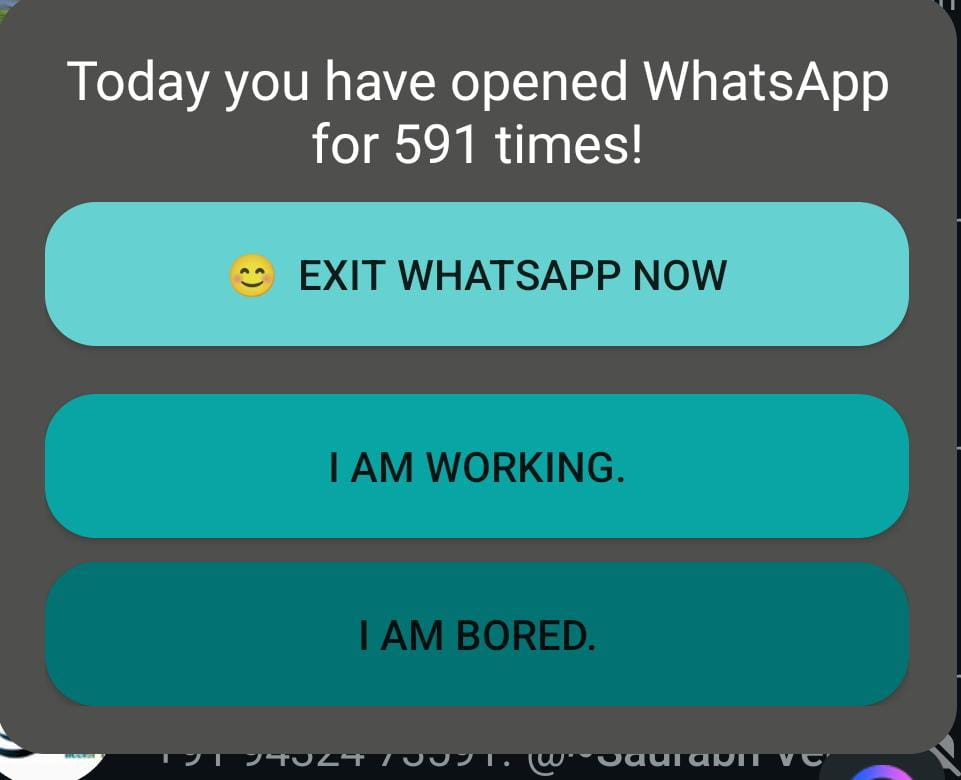
\includegraphics[width=0.5\linewidth]{popup.jpeg}
        \caption{wrong value of launch count}
        \label{fig:enter-label}
    \end{figure}
    \item User is not able to get the usecase of timer.
    \item His response \textbf{Muze ye timer ka kuch samajh he nahi ata, kya use hai iska}
    \item I told him that this timer is for increasing awareness, his response is: \textbf{Nahi, isse kuch farak nahi padta muze, mein switch karke same app open karta hu to phirse counter start hota hai}
        \begin{figure}[H]
        \centering
        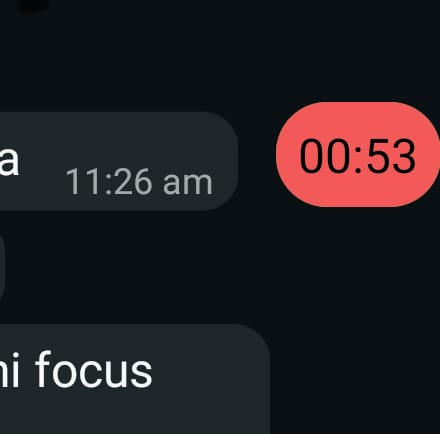
\includegraphics[width=0.5\linewidth]{timer.jpeg}
        \caption{timer running on whatsapp interface}
        \label{fig:enter-label}
    \end{figure}
    \itme User don't like the UI design for side menu bar.
    His reponse is: \textbf{Ye kuch khas nahi dikh raha}
    \begin{figure}[H]
        \centering
        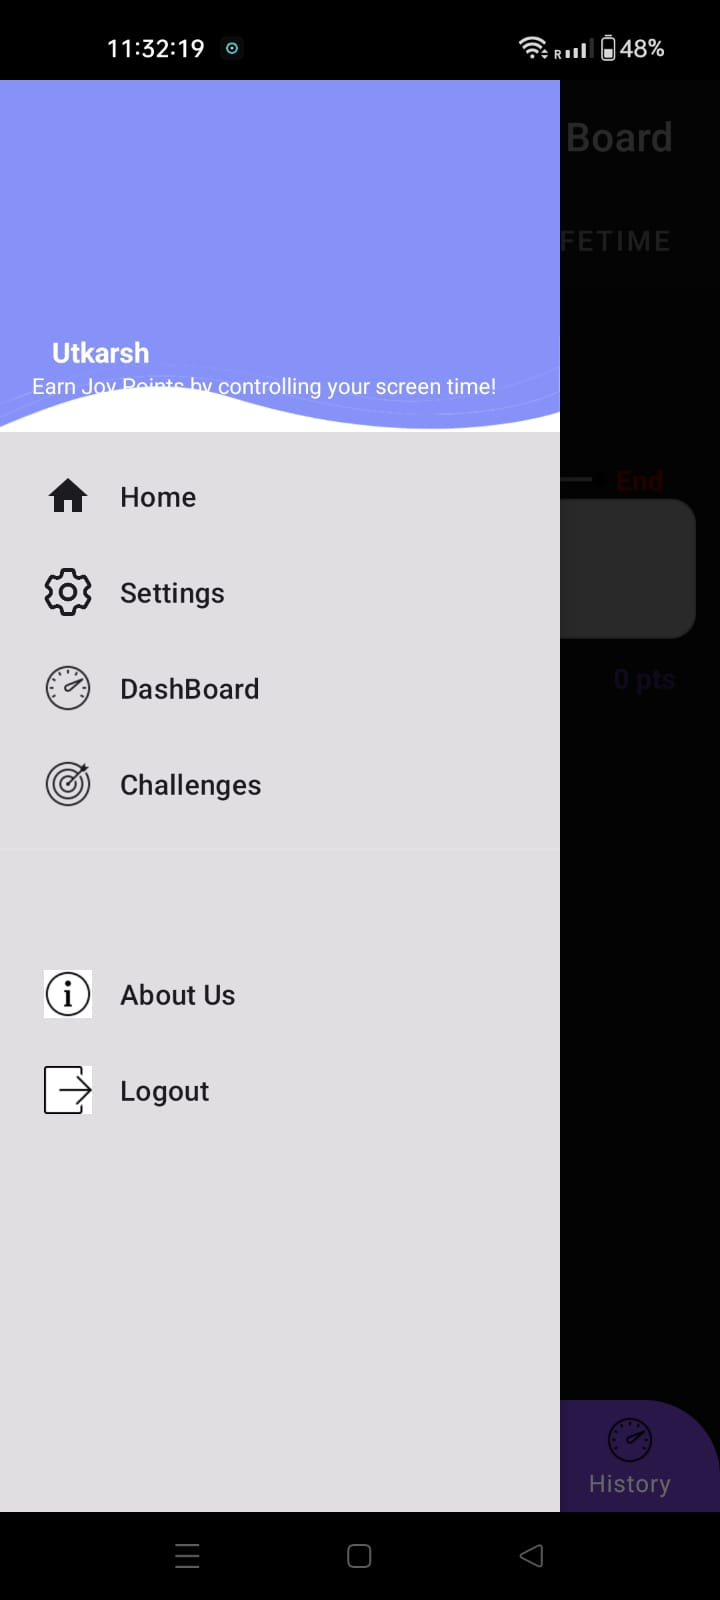
\includegraphics[width=0.5\linewidth]{side_menu.jpeg}
        \caption{side menu bar interface}
        \label{fig:enter-label}
    \end{figure}
\end{enumerate}
\subsection{Pilot Study Plan for Jodo App}

\textbf{Objective}

The purpose of this pilot study is to evaluate the effectiveness of the Jodo app in improving digital wellbeing and productivity among college students. The study aims to measure whether users experience increased focus time, reduced distractions, improved productivity, and better overall study habits.

\subsection{1. Define the Goal}

Clearly define measurable goals before starting the study. Example goals:

\begin{itemize}
    \item Determine whether users increase daily focused study time.
    \item Measure reduction in screen distractions.
    \item Evaluate usability and user experience.
    \item Assess perceived productivity improvement.
\end{itemize}

Example measurable statement:

\textit{Users increase daily focused study time by at least 30 minutes within 7 days of using Jodo.}

\subsection{2. Select Participants}

\begin{itemize}
    \item Recruit 4-5 college students.
    \item Include students from different semesters or departments.
    \item Include both heavy and moderate phone users.
\end{itemize}

This ensures a diverse and relevant sample group aligned with the app’s target audience.

\subsection{3. Decide Study Duration}

\begin{itemize}
    \item Minimum duration: 7 days.
    \item Recommended duration: 14 days.
\end{itemize}

Digital wellbeing improvements require at least one week of consistent usage to observe meaningful trends.

\subsection{4. Pre-Study Survey (Day 0)}

Collect baseline data before participants begin using Jodo. Questions may include:

\begin{itemize}
    \item Average daily study time?
    \item Average daily screen time?
    \item Biggest source of distraction?
    \item Rate productivity (1--10).
    \item Rate stress level (1--10).
\end{itemize}

\subsection{5. Post-Study Survey (After 7 Days)}

Collect feedback and outcome data:

\begin{itemize}
    \item Did Jodo help you focus? (1--10)
    \item Did your study time increase?
    \item Did your screen time reduce?
    \item Which feature helped the most?
    \item What was confusing or difficult?
    \item Would you continue using Jodo? (Yes/No)
    \item Would you recommend it to others? (Yes/No)
\end{itemize}

\subsection{6. Track In-App Metrics}

If available, record:

\begin{itemize}
    \item Number of focus sessions completed
    \item Total focus minutes
    \item App blocking usage
    \item Daily streak consistency
\end{itemize}

This provides objective behavioral data in addition to survey responses.

\subsection{7. Conduct Short User Interviews}

Interview at least 5 participants for deeper insights. Ask:

\begin{itemize}
    \item When did you feel like stopping the app?
    \item What feature was most helpful?
    \item What was frustrating?
    \item What would you use instead if Jodo did not exist?
\end{itemize}

Qualitative feedback often reveals usability improvements and hidden pain points.

\subsection{8. Data Analysis}

Summarize results using a comparison table:

\begin{center}
\begin{tabular}{|c|c|c|}
\hline
Metric & Before & After \\
\hline
Average Study Time & 2 hours & 2.7 hours \\
Average Screen Time & 6 hours & 5 hours \\
Productivity Rating & 5/10 & 7/10 \\
\hline
\end{tabular}
\end{center}

Calculate:
\begin{itemize}
    \item Percentage improvement in focus time
    \item Dropout or uninstall rate
    \item Most frequently appreciated feature
\end{itemize}

\subsection{9. Success Criteria}

The pilot can be considered successful if:

\begin{itemize}
    \item 60\% or more participants want to continue using Jodo.
    \item 50\% or more report increased focus time.
    \item Uninstall rate remains below 30\%.
    \item Clear and actionable feature improvements are identified.
\end{itemize}

\subsection{Conclusion}

This pilot study will help validate the effectiveness, usability, and engagement level of the Jodo app among college students. The insights gained will guide feature improvements and prepare the app for broader deployment.

\section{Feb 23 2026 - Mar 01 2026}
{No. of Hours: 15}
\subsection{To Do}
\begin{enumerate}
    \item Collect log files from various pilot devices and analyze it.
    \item Create script to do data-analysis on pilot's usage data.
    \item Complete post usage interview of the pilots.
     \item Prepare final report  for pilot study.
\end{enumerate}
\subsection{List of task completed}
\begin{enumerate}
    \item Installed app in one more pilot phone(Samsung).
    \item Currently 4 pilots are using the app.
    \item Three pilots completed 7 days on the app.
    \item created github repo (\href{https://github.com/hariom575/MS_Work_logs.git}{link}) for reports.
    \item Created substructure for worklog, RA work, running ms report, running ms pres.
\end{enumerate}
\subsection{Proposed changes for reward model}\href{run:new_proposal.tex}{New Proposal}
\begin{enumerate}
    \item Like forest app they plant trees we can do water cleaning, pollution control stuff, education support for poor people.
    Users focus (Pomodoro / deep work sessions).
    \item For every X minutes completed:
    \begin{enumerate}
\item Fund water purification
 \item Support air pollution control
 \item Sponsor education hours
 \item Plant trees
 \item Waste recycling credits
    \end{enumerate}
   \item  Example IIT Bombay competition:
“Which department funded more education hours this month?”

\end{enumerate}
\subsection{Problem encountered in JoDo}
\begin{enumerate}
    \item App keeps logging out in new devices (pilots).
    \item Bugs in celery scheduler, container keeps stopping after throwing exception related to blocking.
  
\end{enumerate}
\subsection{Feedback Recieved about JoDo}
\begin{enumerate}
    \item Pilot3 is also not comfortable with the HomeScreen.
    \item  Pilot3 removed App as HomeScreen but still keeps using the App.
\end{enumerate}

\subsection{Pilot study user feedbacks}
\begin{enumerate}
    \item Change the default timer value if user click I am bored change it 30 minutes, and user click if am working change to 10 minutes.
\end{enumerate}
\subsection{New Questions}
\begin{enumerate}
    \item Why Being HomeScreen(Fully minimalist and less visual cues) disliked by users?
\end{enumerate}
\section{Feb 26 (last meeting) - Mar 02 2026}
{ \bf No. of Hours: 16}
\subsection{List of Task Completed}
\begin{enumerate}
    \item Create a python Script to retrieve pilot study data from db and generate graphs and insights over them.
    \item Generated pilot Study data analysis report (\href{https://drive.google.com/file/d/10nncQQJaZMth2Gw_ombhluRKVxDVXpRu/view?usp=sharing}{link}).
    \item Collected log file from pilots phone.
    \item In one device found Home screen was crashing due to Integer overflow exception.
    \item App was crashing on Device BootUp in pilots phone.
    \item Prepared new UI design proposal for HomeScreen, Lock Screen and App Drawer.
\end{enumerate}
\subsection{Proposed new UI for JoDo}
\subsubsection{Problem in the current UI}
\begin{enumerate}
    \item It looks like old school.
    \item Progress bar has occupied to much space and it is the main cause of so runtime exceptions in the HomeScreen.
    \item Current UI not properly reflect out Psychology of \textbf{JoDo} as well as \textbf{Digital Minimalism}
\end{enumerate}
\subsubsection{Proposed UI Prototypes:}
\begin{figure}[p]
    \centering
    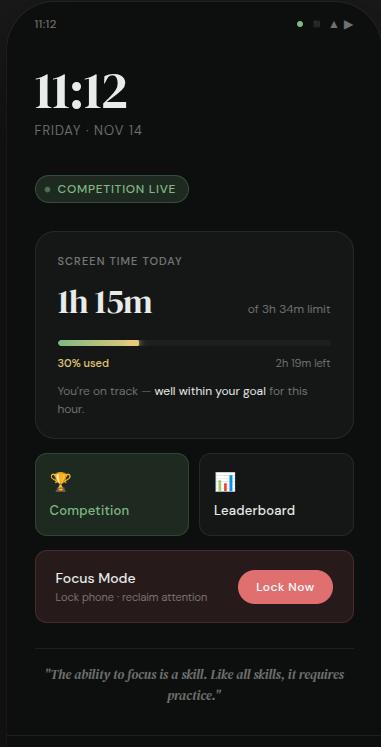
\includegraphics[width=0.45\linewidth,height=0.75\textheight, keepaspectratio]{JoDo new UI design/HomeScreen.png}
    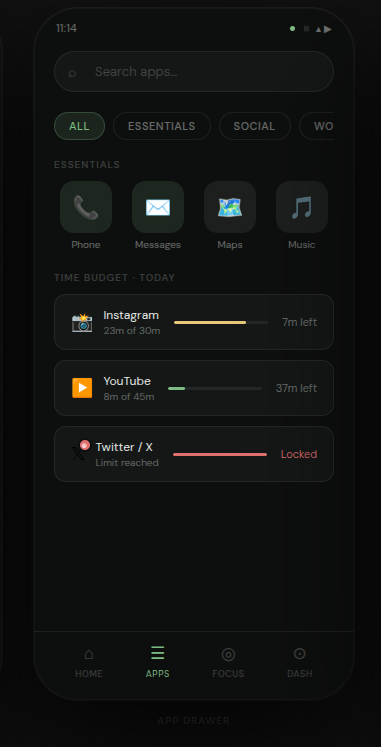
\includegraphics[width=0.45\linewidth, height=0.75\textheight, keepaspectratio]{JoDo new UI design/App_drawer.png}

    \vspace{0.3cm}

    % 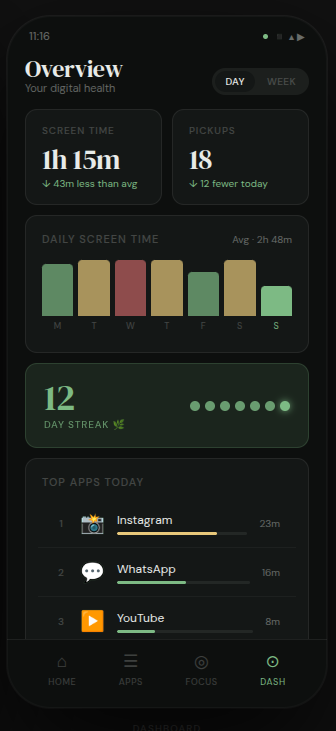
\includegraphics[width=0.45\linewidth]{JoDo new UI design/dashboard.png}
    % 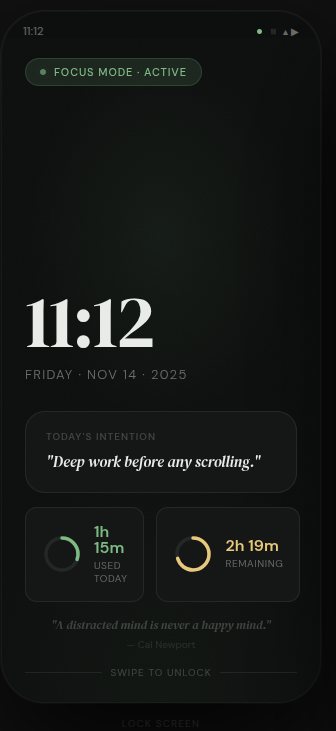
\includegraphics[width=0.45\linewidth]{JoDo new UI design/lock_screen.png}

    \caption{Home-screen(left), App-drawer(right)}
    \label{fig:ui_prototype}
\end{figure}

\newpage
\begin{figure}[p]
    \centering
    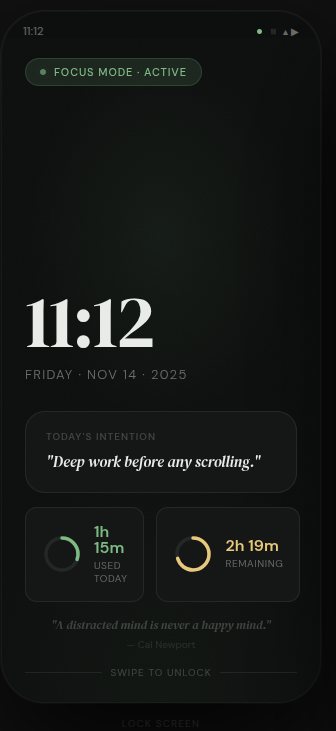
\includegraphics[width=0.45\linewidth,height=0.75\textheight, keepaspectratio]{JoDo new UI design/lock_screen.png}
    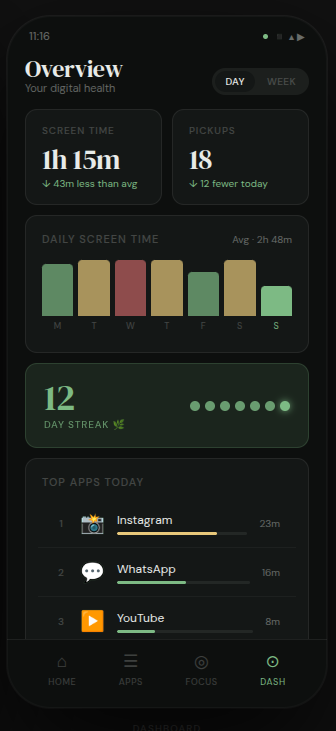
\includegraphics[width=0.45\linewidth, height=0.75\textheight, keepaspectratio]{JoDo new UI design/dashboard.png}

    \vspace{0.3cm}

    % 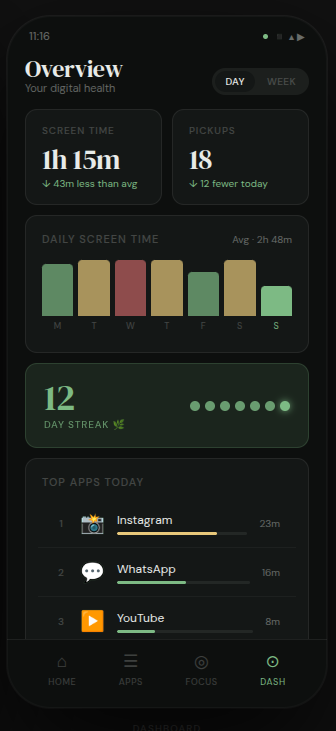
\includegraphics[width=0.45\linewidth]{JoDo new UI design/dashboard.png}
    % 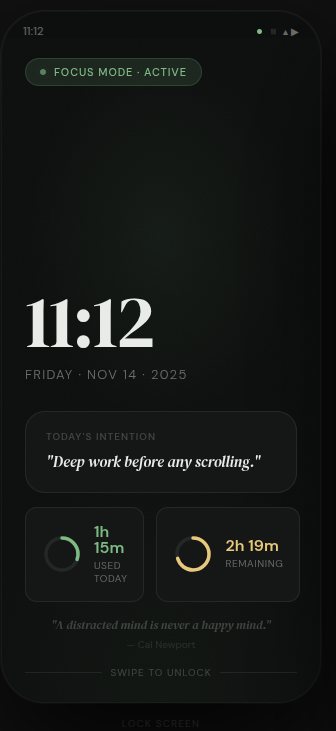
\includegraphics[width=0.45\linewidth]{JoDo new UI design/lock_screen.png}

    \caption{Lock-screen (left), DashBoard (right)}
    \label{fig:ui_prototype}
\end{figure}

\subsection{To Do}
\begin{enumerate}
    \item Complete in person interview of the pilots.
\end{enumerate}
\clearpage
\bibliographystyle{apalike}
\bibliography{reference}


\end{document}
